%%%%%%%%%%%%%%%%%%%%%%%%%%%%%%%%%%%%%%%%%%%%%%%%%%%%%%%%%%%%%%%%%%%%%%%%%%%%%%%
\chapter{Arrasto} % Sem "Experiência 01" ou qualquer outro número
\label{Chap:ExpArrasto}        % para poder trocar a ordem com facilidade
%%%%%%%%%%%%%%%%%%%%%%%%%%%%%%%%%%%%%%%%%%%%%%%%%%%%%%%%%%%%%%%%%%%%%%%%%%%%%%%

\begin{fullwidth}\it
	Realizaremos um experimento para a determinação da velocidade terminal de uma esfera que se move em um fluido dentro de um tubo que faz um ângulo com a horizontal. Através de uma análise dos dados obtidos, verificaremos qual é a dependência da força de arrasto na velocidade. Para isso, veremos as expressões para a força de arrasto com dependência linear e quadrática na velocidade, verificando também como obter a expressão para a velocidade terminal em função do ângulo de inclinação. Utilizaremos os conceitos de medidas, algarismos significativos, gráficos, regressão linear, e linearização.
\end{fullwidth}

%%%%%%%%%%%%%%%%%%%%%%%%%%%%%%%%%%%%%%%%%%%%%%%%%%%%%%%%%%%%%%%%%%%%%%%%%%%%%%%
\section{Força de Arrasto}
%%%%%%%%%%%%%%%%%%%%%%%%%%%%%%%%%%%%%%%%%%%%%%%%%%%%%%%%%%%%%%%%%%%%%%%%%%%%%%%

Quando nos deslocamos em uma piscina, verificamos que há uma grande força que se opõe ao nosso movimento. Mesmo ao nos deslocarmos no ar, um fluido muito menos denso que a água, podemos perceber que em velocidades elevadas existe o mesmo tipo de força que se opõe ao movimento. 

Em ambos os casos é possível perceber que há uma relação entre a velocidade do deslocamento e a intensidade da força. A descrição dsta força ---~que recebe o nome de \emph{Força de Arrasto}~--- é, no entanto, bastante complicada. Em deslocamentos no ar, com velocidades moderadas, a expressão para a força é dada por
\begin{equation}
	F_a = \frac{1}{2} C\rho A v^2,
\end{equation}
%
onde
\begin{itemize}
	\item $C$ é um parâmetro adimensional conhecido como \emph{coeficiente de arrasto} e cujo valor é determinado experimentalmente. Seu valor depende de propriedades como a forma eas características da superfície do objeto. Além disso, seu valor pode variar com a velocidade. Seus valores típicos estão compreendidos na faixa entre \np{0,4} e \np{1,0}.
	\item $A$ é a área de seção reta do objeto. Tal área pode ser interpretada como a sombra do objeto ao ser iluminado por uma fonte de luz distante e cuja direção dos raios luminosos seja a mesma do movimento.
	\item $\rho$ é a densidade do meio onde o objeto se desloca.
	\item Finalmente, $v^2$ representa o quadrado da velocidade do objeto em relação ao meio.
\end{itemize}

\pagebreak

Esse conjunto de parâmetros às vezes é escrito de uma maneira compacta utilizando a notação $b_2 = C\rho A /2$ e a força de arrasto como
\begin{equation}
	F_a = b_2 v^2.
\end{equation}

Muitas vezes, porém, temos fluidos e/ou regimes de velocidade para os quais a expressão acima falha. A força de arrasto que atua sobre o casco de um navio, por exemplo, é em geral descrita através da equação\footnote{As constantes $b_1$ e $b_2$ em geral não têm o mesmo valor.}
\begin{align}
	F_a &= 6\pi\eta R v \\
	&= b_1 v.
\end{align}

Podemos dizer, portanto, que existem pelo menos duas hipóteses para a descrição da força de arrasto que age sobre um corpo. Vamos analisar um experimento e realizar um teste para determinar qual hipótese é a mais adequada.

%%%%%%%%%%%%%%%%%%%%%%%%%%%%%%%%%%%%%%%%%%%%
\section{Força de arrasto e velocidade terminal}
\label{SecaoF_a}
%%%%%%%%%%%%%%%%%%%%%%%%%%%%%%%%%%%%%%%%%%%%

Vamos analisar o movimento de uma esfera que se desloca dentro de um tubo preenchido com um fluido (água) e está sujeito a uma força de arrasto. Vamos considerar que o tubo está inclinado de um ângulo $\theta$ em relação à horizontal. Nesse caso, atuam sobre a esfera a força peso, a força normal e a força de arrasto (veja a Figura~\ref{DiagramaEsfera}).

\begin{marginfigure}
	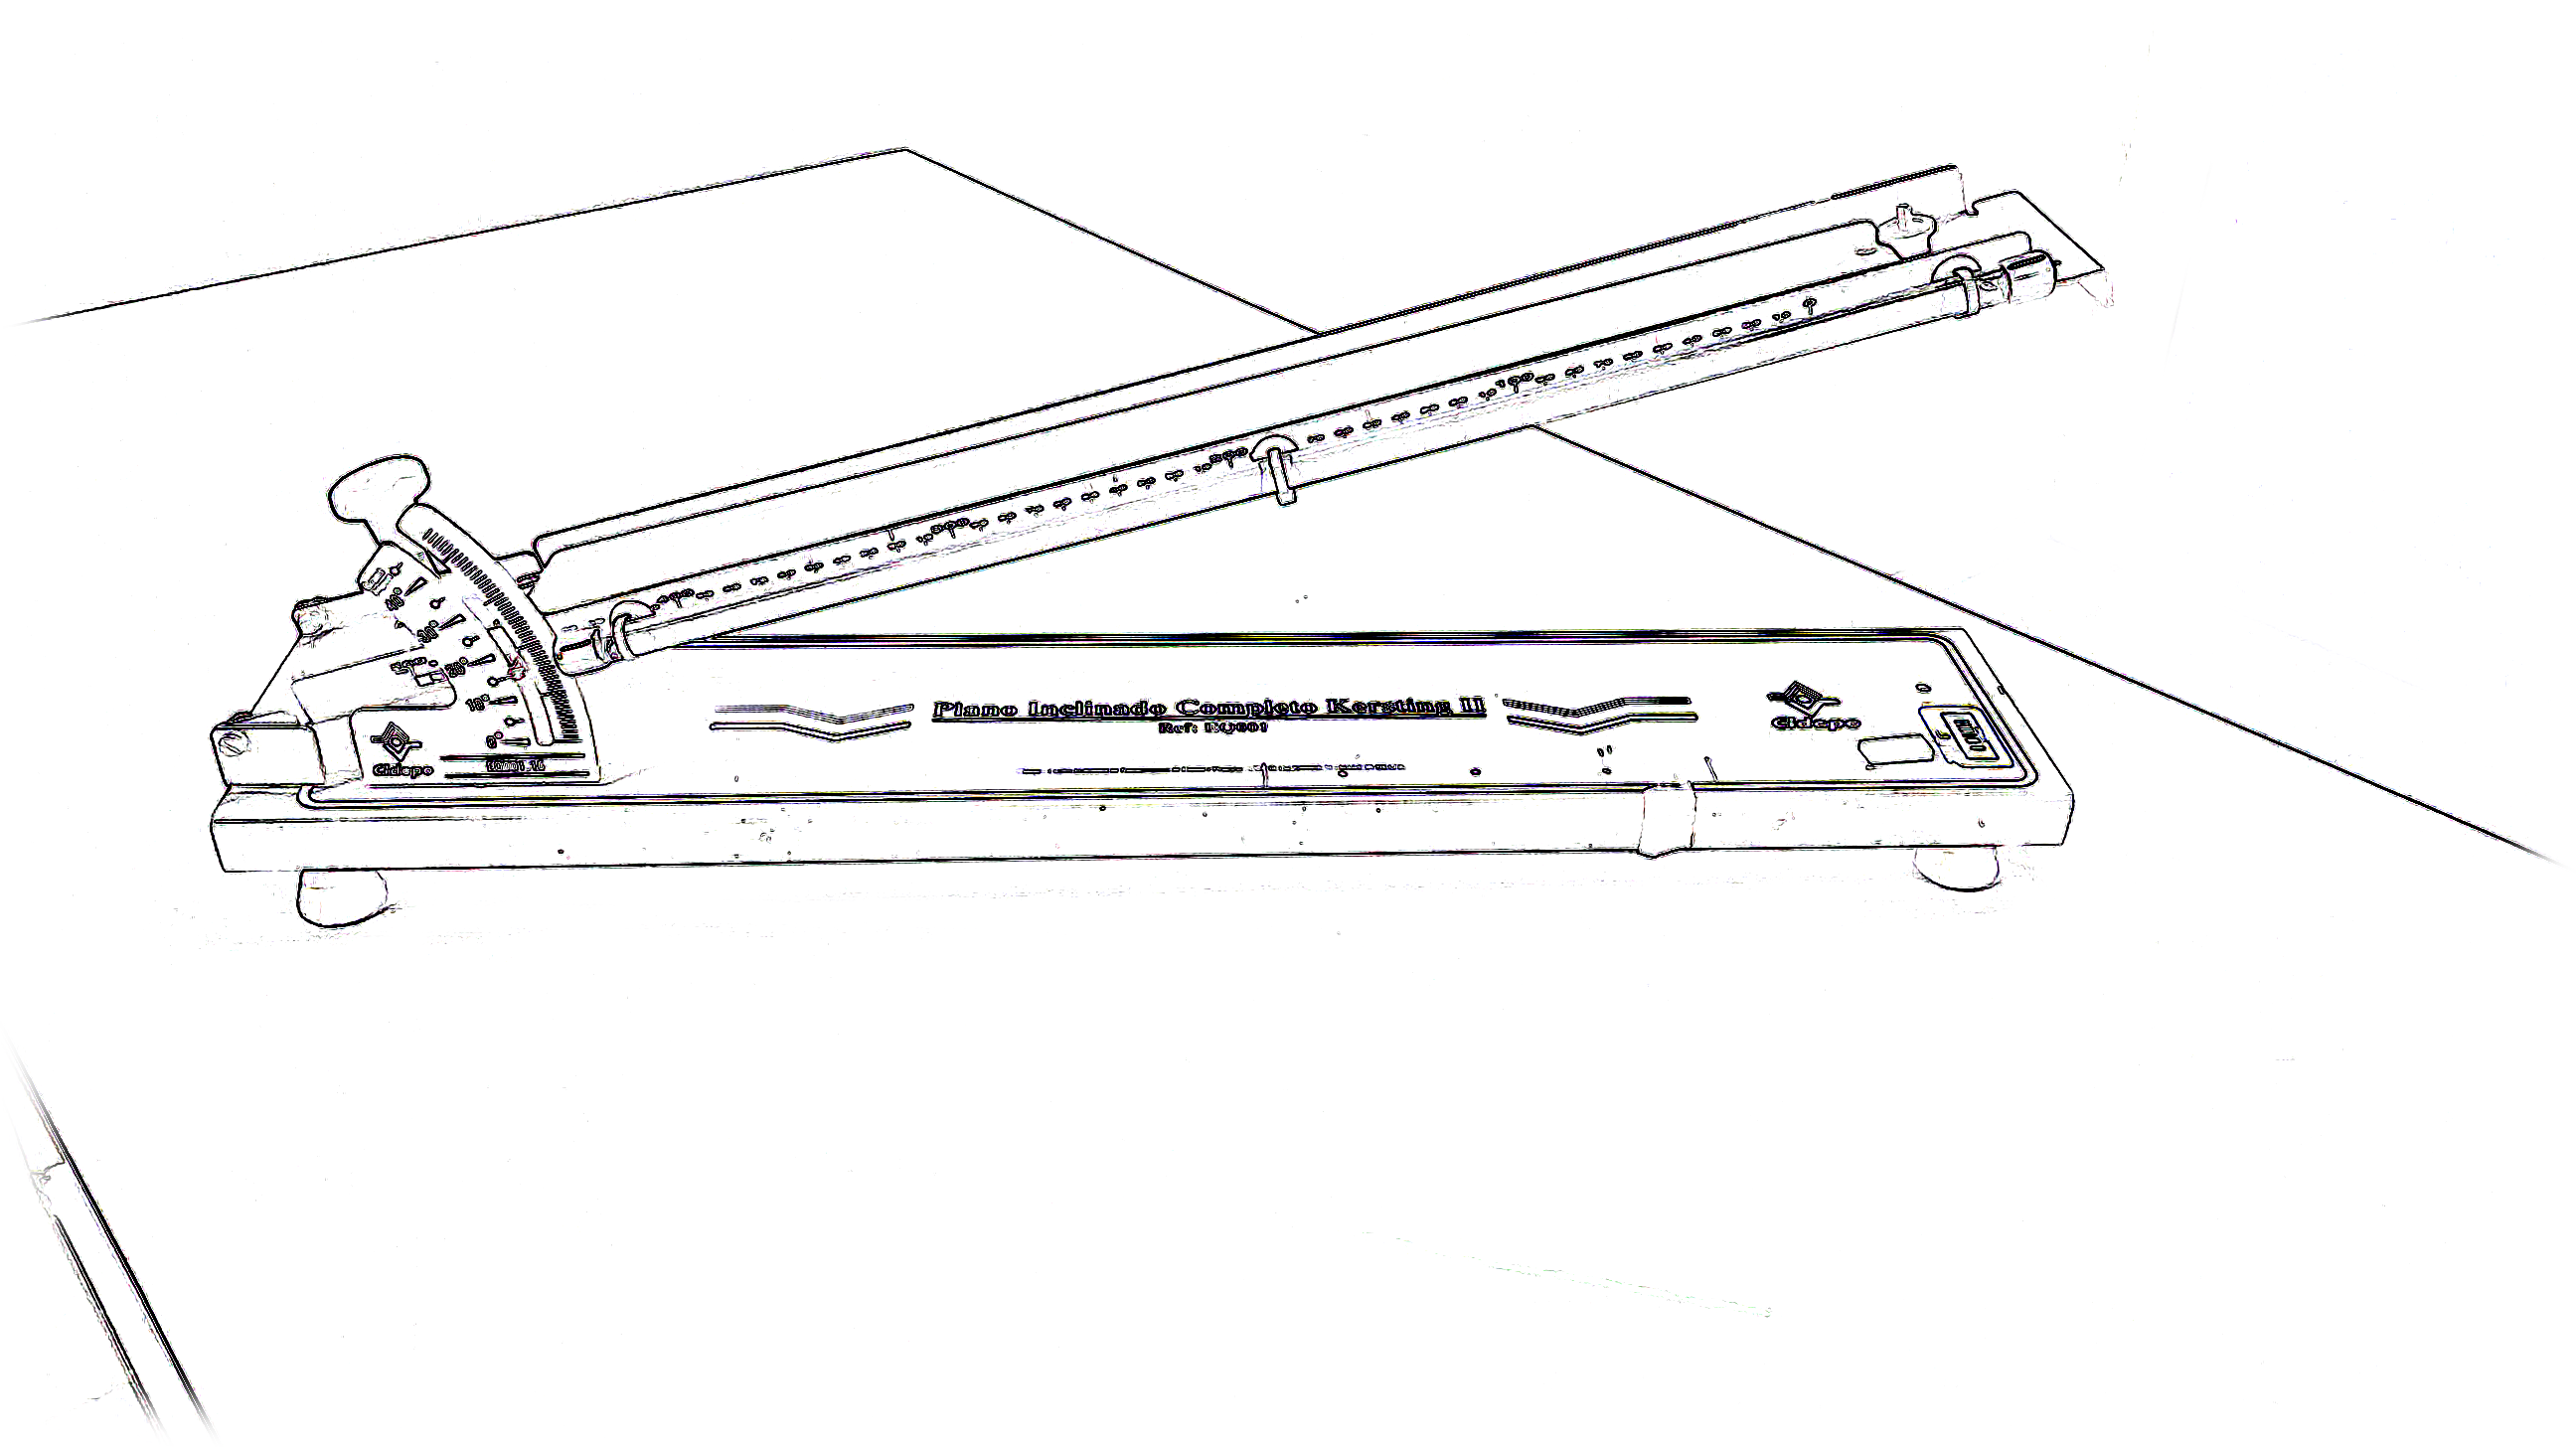
\includegraphics[width=\textwidth]{Ilustrations/Arrasto.png}
	\caption{Plano inclinado com tubo contendo fluido e uma esfera de aço que pode se deslocar.}
\end{marginfigure}

\begin{marginfigure}
\centering
\begin{tikzpicture}[>=Stealth, scale = 1.25]
	\begin{scope}[rotate=30]
%   	\usetikzlibrary{calc}
%   	\def\centerarc[#1](#2)(#3:#4:#5)% [draw options] (center) (initial angle:final angle:radius)
%   	{ \draw[#1] ($(#2)+({#5*cos(#3)},{#5*sin(#3)})$) arc (#3:#4:#5) node[below]{$\theta$}; }
	
	    \draw[dotted,very thin, <-] (-2,0) node[below] {$x$} -- (2,0);
	    \draw[dotted,very thin, ->] (0,-1.5) coordinate (B) -- (0,2) node[left]{$y$};
	    
	    \draw[->] (0,0) coordinate (O) -- node[above right]{$\vec{N}$} (0,0.866025404);
	    \draw[->, dashed] (0,0) -- (-0.5,0) node[above=3pt]{$P_x$};
	    \draw[->, dashed] (0,0) -- (0, -0.866025404) node[right]{$P_y$};
	    \draw[->] (0,0) -- node[below right]{$\vec{F}_a$} (0.5,0);
	    \draw[densely dotted] (-0.5,0) -- (-0.5,-0.866025404);
	    \draw[densely dotted] (-0.5,-0.866025404) -- (0, -0.866025404);
%	    \draw (-0.230940108,-0.4) arc (240:270:0.4619) node[below]{$\theta$};
	\end{scope}
	\draw[fill] (0,0) circle[radius=0.1];
	\draw[->] (0,0) -- (0,-1) node[below left]{$\vec{P}$} coordinate (A);
	
	\pic[draw, "$\theta$", angle radius = 6mm, angle eccentricity = 1.3]{angle=A--O--B};
	
\end{tikzpicture}
\caption{Diagrama de corpo livre da esfera que se desloca dentro do tubo.}
\label{DiagramaEsfera}
\end{marginfigure}

Verificamos para o eixo $y$ que a força normal deve ser equilibrada pela componente $y$ da força peso, pois o objeto não se desloca no eixo $y$ e, portanto, sua aceleração deve ser zero. Já para o eixo $x$, verificamos que
\begin{align}
    F_{R,x} &= m a_x \\
	P_x - F_{a,x} &= ma_x.
\end{align}
%
Substituindo $F_a = b_n v^{n}$, onde $n=1$~ou~$2$ ---~de acordo com as hipóteses discutidas na seção anterior~---, temos
\begin{equation}
	P_x - b_n v^n = ma_x.
\end{equation}

Verificamos então que conforme a velocidade do objeto aumenta, a força de arrasto também aumenta. Isso dá origem a uma \emph{velocidade limite}, isto é, uma velocidade máxima para a qual a força de arrasto equilibra completamente a componente da força peso na direção do eixo $x$. Temos então uma aceleração nula e, portanto, uma velocidade constante. O valor da velocidade terminal pode ser calculado através de
\begin{equation}
	P_x - b_n v_t^n = 0,
\end{equation}
%
ou, substituindo $P_x = Mg\sen\theta$,
\begin{equation}
	v_t^n = \frac{Mg}{b_n}\,\sen\theta.
\end{equation}

A partir do resultado acima, vemos que a velocidade terminal só depende do ângulo $\theta$ de inclinação do tubo, uma vez que os demais parâmetros são constantes. Substituindo os valores de $n$ na equação acima, temos duas hipóteses
\begin{align}
	v_t =\frac{Mg}{b_1}\sen\theta, \qquad\textrm{Hipótese 1} \\
	v_t^2 =\frac{Mg}{b_2}\sen\theta, \qquad\textrm{Hipótese 2.}
\end{align}

Como a velocidade terminal é constante, podemos estabelecer uma posição inicial e uma posição final no tubo cujo tempo de deslocamento possa ser cronometrado. Utilizando uma distância $\Delta x$ fixa, temos então que
\begin{equation}
	v_t = \Delta x / \Delta t.
\end{equation}
%
É importante notar que o objeto já deve ter atingido a velocidade limite antes da posição inicial para que a equação acima seja válida.

%%%%%%%%%%%%%%%%%%%%%%%%%%%%%%%%%%%%%%%%%%%%%%%%%%%%
\subsection{Linearização e teste das duas hipóteses}
%%%%%%%%%%%%%%%%%%%%%%%%%%%%%%%%%%%%%%%%%%%%%%%%%%%%

Para decidirmos qual das hipóteses acima melhor descreve a força de arrasto no experimento, vamos utilizar o coeficiente $r^2$. Para tanto, vamos comparar as duas hipóteses com a equação da reta:
\begin{description}
	\item[Hipótese 1:] Temos nesse caso a seguinte relação entre a equação que rege o fenômeno e a equação da reta:
		\begin{align}
			y &= v_t \\
			A &= 0 \\
			B &= Mg/b_1 \\
			x &= \sen\theta
		\end{align}

	\item[Hipótese 2:] Nesse caso, temos
		\begin{align}
			y &= v_t^2 \\
			A &= 0 \\
			B &= Mg/b_2 \\
			x &= \sen\theta
		\end{align}
\end{description}

%%%%%%%%%%%%%%%%%%%%%%%%%%%%%%%%%%%%%%%%%%%%%%%%%%%%%%%%%%%%%%%%%%%%%%%%%%%%%%%
\section{Experimento}
%%%%%%%%%%%%%%%%%%%%%%%%%%%%%%%%%%%%%%%%%%%%%%%%%%%%%%%%%%%%%%%%%%%%%%%%%%%%%%%

Considerando o movimento de uma esfera em um plano inlinado e sujeita a uma força de arrasto, vamos verificar o tempo necessário para que a ela percorra uma distância preestabelecida, porém para diversos ângulos de inclinação distintos. Para que possamos determinar a velocidade de maneira simples, é necessário que a esfera tenha atingido a velocidade terminal antes de passar pela posição que marca o início do intervalo para o qual mediremos a distância e o tempo. Isso significa que a esfera deve ser solta a partir de um ponto que preceda o ponto inicial por alguns centímetros.\footnote[][-3cm]{Como a esfera tem massa pequena e o fluido é razoavelmente viscoso, a distância necessária é pequena, por volta de \np[cm]{3,00} são suficientes.}

%%%%%%%%%%%%%%%%%%%%%%
\subsection{Objetivos}
%%%%%%%%%%%%%%%%%%%%%%

\begin{itemize}
     \item Verificar a relação entre a força de arrasto e a velocidade;
	 \item Linearizar os conjuntos de dados obtidos e obter os valores de $A$ e $B$ das equações da retas correspondentes;
     \item Elaborar um gráfico $v_t \times \sen\theta$ dos pontos experimentais e adicional a ele a reta obtida através da regressão linear;
	 \item Elaborar um gráfico $v_t^2 \times \sin\theta$ dos pontos experimentais e adicionar a ele a reta obtida através da regressão linear.
\end{itemize}

%%%%%%%%%%%%%%%%%%%%%%%%%%%%%%%%%%%%%%%%%%%%%%%%%%%%%%%%%%%%%%%%%%%%%%%%%%%%%%%
\section{Material Necessário}
%%%%%%%%%%%%%%%%%%%%%%%%%%%%%%%%%%%%%%%%%%%%%%%%%%%%%%%%%%%%%%%%%%%%%%%%%%%%%%%

\begin{itemize}
	\item Plano inclinado;
	\item Cronômetro;
	\item Ímã;
	\item Régua.
\end{itemize}

%%%%%%%%%%%%%%%%%%%%%%%%%%%%%%%%%%%%%%%%%%%%%%%%%%%%%%%%%%%%%%%%%%%%%%%%%%%%%%%
\section{Procedimento Experimental}
%%%%%%%%%%%%%%%%%%%%%%%%%%%%%%%%%%%%%%%%%%%%%%%%%%%%%%%%%%%%%%%%%%%%%%%%%%%%%%%

\begin{enumerate}
	\item Ajuste o plano inclinado para um ângulo de \np[\tcdegree]{5,0}.
	\item Estabeleça o $x_i$ como \np[cm]{10,00}.
	\item Estabeleça o $x_f$ como \np[cm]{40,00}.
	\item Use o ímã para levar a esfera até a posição mais alta do tubo.
	\item Solte a esfera e cronometre o tempo necessário para atravessar a distância entre $x_i$ e $x_f$. Anote o valor na tabela.
	\item Repita a tomada de tempo mais duas vezes para este ângulo.
	\item Aumente o ângulo em \np[\tcdegree]{5,0} e repita os passos acima. Realize este procedimento até atingir o ângulo de \np[\tcdegree]{40,0}.
\end{enumerate}

%%%%%%%%%%%%%%%%%%%%%%%%%%%%%%%%%%%%%%%%%%%%%%%%%%%%%%%%%%%%%%%%%%%%%%%%%%%%%%%
%%%%%%%%%%%%%%%%%%%%%%%%%%%%%%%%%%%%%%%%%%%%%%%%%%%%%%%%%%%%%%%%%%%%%%%%%%%%%%%
%%%%%%%%%%%%%%%%%%%%%%%%%%%%%%%%%%%%%%%%%%%%%%%%%%%%%%%%%%%%%%%%%%%%%%%%%%%%%%%
%%%%%%%%%%%%%%%%%%%%%%%%%%%%%%%%%%%%%%%%%%%%%%%%%%%%%%%%%%%%%%%%%%%%%%%%%%%%%%%
\cleardoublepage

\noindent{}{\huge\textit{Arrasto}}

\vspace{15mm}

\begin{fullwidth}
\noindent{}\makebox[0.6\linewidth]{Turma:\enspace\hrulefill}\makebox[0.4\textwidth]{  Data:\enspace\hrulefill}
\vspace{5mm}

\noindent{}\makebox[0.6\linewidth]{Aluno(a):\enspace\hrulefill}\makebox[0.4\textwidth]{  Matrícula:\enspace\hrulefill}

\noindent{}\makebox[0.6\linewidth]{Aluno(a):\enspace\hrulefill}\makebox[0.4\textwidth]{  Matrícula:\enspace\hrulefill}

\noindent{}\makebox[0.6\linewidth]{Aluno(a):\enspace\hrulefill}\makebox[0.4\textwidth]{  Matrícula:\enspace\hrulefill}

\noindent{}\makebox[0.6\linewidth]{Aluno(a):\enspace\hrulefill}\makebox[0.4\textwidth]{  Matrícula:\enspace\hrulefill}

\noindent{}\makebox[0.6\linewidth]{Aluno(a):\enspace\hrulefill}\makebox[0.4\textwidth]{  Matrícula:\enspace\hrulefill}
\end{fullwidth}

\vspace{5mm}

%%%%%%%%%%%%%%%%%%%%%%%%%%%%%%%%%%%%%%%%%%%%%%%%%%%%%%%%%%%%%%%%%%%%%%%%%%%%%%%
\section{Questionário}
%%%%%%%%%%%%%%%%%%%%%%%%%%%%%%%%%%%%%%%%%%%%%%%%%%%%%%%%%%%%%%%%%%%%%%%%%%%%%%%

\begin{question}[type={exam}]{1}
Apresente os resultados de maneira clara e organizada. Mostre os cálculos requisitados de maneira clara e sucinta, evidenciando o raciocínio desenvolvido.
\end{question}

\begin{question}[type={exam}]{1}
Preencha as colunas de dados das tabelas com o número adequado de algarismos significativos e unidades.
\end{question}


\begin{question}[type={exam}]{3}
Elabore um gráfico $v_t \times \sen\theta$ dos pontos experimentais e um gráfico de $v_t^2 \times \sen\theta$.
\end{question}

\begin{question}[type={exam}]{3}
Através dos gráficos elaborados no item anterior, para ambos os conjuntos de dados, obtenha os valores de $A$, $B$ e $r^2$ da melhor reta correspondente (a reta da regressão linear). Adicione essa reta ao gráfico e coloque a equação da reta, juntamente com o coeficiente $r^2$ na legenda.
\end{question}

\begin{question}[type={exam}]{2}
Através da análise do coeficiente de dispersão linear $r^2$, indique qual das hipóteses discutidas na Seção~\ref{SecaoF_a} melhor descreve o fenômeno.
\end{question}
\vfill

%%%%%%%%%%%%%%%%%%%%%%%%%%%%%%%%%%%%%%%%%%%%%%%%%%%%%%%%%%%%%%%%%%%%%%%%%%%%%%%
\pagebreak
\section{Tabelas}
%%%%%%%%%%%%%%%%%%%%%%%%%%%%%%%%%%%%%%%%%%%%%%%%%%%%%%%%%%%%%%%%%%%%%%%%%%%%%%%

\begin{table*}[!h]
\centering
\begin{tabular}{lp{25mm}p{25mm}p{25mm}p{25mm}p{25mm}l}
\toprule
	& \multicolumn{2}{l}{\textbf{Posições inicial e final}} \\
	\cmidrule{2-3}
	& $x_i$ \cellcolor[gray]{0.89} & \cellcolor[gray]{0.92} \\
	& $x_f$ \cellcolor[gray]{0.95} & \cellcolor[gray]{0.97} \\
	\cmidrule{2-3}
\\
	& \multicolumn{6}{l}{\textbf{Dados experimentais}} \\
	\cmidrule{2-6}
	& $t_1$ & $t_2$ & $t_3$ & $\mean{t}$ & $\theta$ & \\
	\cmidrule{2-6}
	& \cellcolor[gray]{0.89} & \cellcolor[gray]{0.92} & \cellcolor[gray]{0.89} & \cellcolor[gray]{0.92} & \cellcolor[gray]{0.89} \\
	& \cellcolor[gray]{0.95} & \cellcolor[gray]{0.97} & \cellcolor[gray]{0.95} & \cellcolor[gray]{0.97} & \cellcolor[gray]{0.95} \\
	& \cellcolor[gray]{0.89} & \cellcolor[gray]{0.92} & \cellcolor[gray]{0.89} & \cellcolor[gray]{0.92} & \cellcolor[gray]{0.89} \\
	& \cellcolor[gray]{0.95} & \cellcolor[gray]{0.97} & \cellcolor[gray]{0.95} & \cellcolor[gray]{0.97} & \cellcolor[gray]{0.95} \\
	& \cellcolor[gray]{0.89} & \cellcolor[gray]{0.92} & \cellcolor[gray]{0.89} & \cellcolor[gray]{0.92} & \cellcolor[gray]{0.89} \\
	& \cellcolor[gray]{0.95} & \cellcolor[gray]{0.97} & \cellcolor[gray]{0.95} & \cellcolor[gray]{0.97} & \cellcolor[gray]{0.95} \\
	& \cellcolor[gray]{0.89} & \cellcolor[gray]{0.92} & \cellcolor[gray]{0.89} & \cellcolor[gray]{0.92} & \cellcolor[gray]{0.89} \\
	& \cellcolor[gray]{0.95} & \cellcolor[gray]{0.97} & \cellcolor[gray]{0.95} & \cellcolor[gray]{0.97} & \cellcolor[gray]{0.95} \\
	& \cellcolor[gray]{0.89} & \cellcolor[gray]{0.92} & \cellcolor[gray]{0.89} & \cellcolor[gray]{0.92} & \cellcolor[gray]{0.89} \\
	& \cellcolor[gray]{0.95} & \cellcolor[gray]{0.97} & \cellcolor[gray]{0.95} & \cellcolor[gray]{0.97} & \cellcolor[gray]{0.95} \\
	& \cellcolor[gray]{0.89} & \cellcolor[gray]{0.92} & \cellcolor[gray]{0.89} & \cellcolor[gray]{0.92} & \cellcolor[gray]{0.89} \\
	& \cellcolor[gray]{0.95} & \cellcolor[gray]{0.97} & \cellcolor[gray]{0.95} & \cellcolor[gray]{0.97} & \cellcolor[gray]{0.95} \\
	\cmidrule{2-6}
\\
	& \multicolumn{2}{l}{\textbf{Dados para o gráfico}} \\
	\cmidrule{2-3}
	& $v_t$ & $\sen\theta$ \\
	\cmidrule{2-3}
	& \cellcolor[gray]{0.89} & \cellcolor[gray]{0.92} \\
	& \cellcolor[gray]{0.95} & \cellcolor[gray]{0.97} \\
	& \cellcolor[gray]{0.89} & \cellcolor[gray]{0.92} \\
	& \cellcolor[gray]{0.95} & \cellcolor[gray]{0.97} \\
	& \cellcolor[gray]{0.89} & \cellcolor[gray]{0.92} \\
	& \cellcolor[gray]{0.95} & \cellcolor[gray]{0.97} \\
	& \cellcolor[gray]{0.89} & \cellcolor[gray]{0.92} \\
	& \cellcolor[gray]{0.95} & \cellcolor[gray]{0.97} \\
	& \cellcolor[gray]{0.89} & \cellcolor[gray]{0.92} \\
	& \cellcolor[gray]{0.95} & \cellcolor[gray]{0.97} \\
	& \cellcolor[gray]{0.89} & \cellcolor[gray]{0.92} \\
	& \cellcolor[gray]{0.95} & \cellcolor[gray]{0.97} \\
	\cmidrule{2-3}
\bottomrule
\end{tabular}
\caption[][5mm]{Dados para o movimento efetuado pela esfera sob ação da gravidade e do arrasto.}
\label{TabelaDados}
\end{table*}
